\documentclass[10pt,twocolumn,letterpaper]{article}
\usepackage{graphicx}
\usepackage{amsmath}
\usepackage{amssymb}
\usepackage{booktabs}
\usepackage{float}
\usepackage[pagebackref,breaklinks,colorlinks]{hyperref}
\usepackage[capitalize]{cleveref}
\usepackage{abstract} % Add this package for abstract formatting
\usepackage{afterpage}
\usepackage{subcaption}  % Add this package for subfigures
\setlength{\topmargin}{-0.7in}
\setlength{\textheight}{9.5in} 
\setlength{\columnsep}{20pt}
\crefname{section}{Sec.}{Secs.}
\Crefname{section}{Section}{Sections}
\Crefname{table}{Table}{Tables}
\crefname{table}{Tab.}{Tabs.}



\begin{document}

\title{Real-time Domain Adaptation in Semantic Segmentation}

\author{Ianniello Luca, 
Martone Raffaele,
Sirica Antonio\\}


%%%%%%%%% ABSTRACT
\twocolumn[
\maketitle
\begin{@twocolumnfalse}
\begin{abstract}
\textit{ 
    This study addresses the challenge of real-time domain adaptation in semantic segmentation, focusing on bridging the performance gap between source and target domains. Leveraging the LoveDA dataset, which encompasses both rural and urban environments, we evaluate the performance of state-of-the-art models, including DeepLabV2 and PIDNet, under domain adaptation settings. We experiment with different configurations, loss functions, and optimizers to assess their impact. Furthermore, we explore a range of adaptation techniques, such as data augmentation, adversarial learning, domain adaptation via cross-domain mixed sampling (DACS), Prototype-based Efficient MaskFormer (PEM), and unpaired image-to-image translation using CycleGAN. Our findings highlight the strengths and limitations of these methods in improving segmentation performance across domains while maintaining computational efficiency. The GitHub repository for this project can be found at: \href{https://github.com/LucaIanniello/AML2024.git}{https://github.com/LucaIanniello/AML2024.git} \cite{amlproject2024}.
}
\end{abstract}
\vspace{1.2em}
\end{@twocolumnfalse}
]


%%%%%%%%% BODY TEXT
\section{Introduction}
\label{sec:intro}

Semantic segmentation is a fundamental task in computer vision that involves partitioning an image into semantically meaningful regions, typically corresponding to different object classes. This task is crucial for various applications, including autonomous driving, medical imaging, and remote sensing. Recent advancements in deep learning have significantly improved the performance of semantic segmentation models \cite{hao2020brief}. 

While deep learning models such as DeepLab \cite{chen2017deeplab} and PIDNet \cite{feng2021pidnet} have achieved remarkable performance on benchmark datasets, their generalization to unseen domains remains a significant obstacle. Domain shifts, arising from differences in image characteristics, environments, and data distributions, often result in substantial performance degradation.

Domain adaptation aims to bridge the performance gap between source and target domains, enabling models trained on one domain to generalize effectively to another. The LoveDA dataset \cite{wang2021loveda}, with its distinct rural and urban domain settings, provides a robust benchmark for evaluating domain adaptation techniques in semantic segmentation. 

This project investigates real-time domain adaptation techniques for semantic segmentation, focusing on the LoveDA dataset. We evaluate state-of-the-art models, such as DeepLabv2 and PIDNet, under various domain adaptation scenarios. Specifically, we analyze the challenges of adapting models from rural to urban domains and vice versa, and we explore solutions including data augmentation, adversarial training \cite{tsai2018advlearning}, image-to-image translation approaches (DACS) \cite{tranheden2021dacs}, real-time networks (PEM) \cite{cavagnero2024pem}, and style transfer preprocessing models, like CycleGAN \cite{zhu2020cyclegan}. By experimenting with these approaches, we aim to identify effective methods for improving domain adaptation performance while maintaining real-time capabilities.

\section{Related Work}
\label{sec:related}

In this section, we provide an overview of the state-of-the-art models and techniques for semantic segmentation and domain adaptation used to implement the basic structure of our project.

\subsection{DeepLabV2}

DeepLab has played a important role in advancing semantic segmentation by overcoming key challenges in traditional deep convolutional neural networks (DCNNs), including resolution loss, scale variability, and poor boundary localization \cite{chen2017deeplab}. DeepLab V2 specifically addresses these issues through three major contributions: atrous convolution, Atrous Spatial Pyramid Pooling (ASPP), and Fully Connected Conditional Random Fields (CRFs).
Atrous convolution, or dilated convolution, mitigates resolution loss by expanding the receptive field without increasing computational costs or reducing spatial resolution. This enables accurate pixel-level predictions while preserving fine details. To tackle scale variability, the ASPP module aggregates multi-scale contextual information using parallel atrous convolutions with varying dilation rates, ensuring robustness to objects appearing at different sizes. Finally, Fully Connected CRFs refine segmentation results by modeling pixel relationships based on spatial proximity and color similarity. This post-processing step enhances boundary delineation and recovers intricate object edges.
By addressing these core challenges, DeepLab V2 has become a benchmark framework in semantic segmentation, achieving high-resolution predictions, robust multi-scale representations, and precise boundary localization. Its innovations have significantly influenced subsequent research, setting a new standard for segmentation methodologies.
DeepLabv2 was used in our project in the first experiments to evaluate its performance in domain adaptation scenarios and to better understand the behaviour of a classic segmentation network.

\subsection{PIDNet}

PIDNet is a real-time semantic segmentation network inspired by Proportional-Integral-Derivative (PID) controllers, which are commonly used in control systems to achieve precision and stability \cite{feng2021pidnet}. By drawing from PID control theory, PIDNet introduces a unique architecture with three specialized branches—P (proportional), I (integral), and D (derivative)—each capturing distinct and complementary information. The P-branch focuses on preserving spatial details, the I-branch aggregates global contextual information, and the D-branch enhances boundary precision. This design allows PIDNet to achieve a balance between low-latency processing and high segmentation quality. Particularly effective in real-time applications such as autonomous driving and robotics, PIDNet delivers state-of-the-art performance while maintaining a lightweight structure. This efficiency makes it suitable for resource-constrained environments without significant compromise in accuracy, showcasing its versatility and practical utility across diverse domains. PIDNet is the basic model we will use for our experiments and we have also implemented some changes to improve its performance in domain adaptation scenarios. These changes will be discussed in the following sections.

\subsection{LoveDa Dataset}

The dataset used in our experiments is the LoveDA dataset. The LoveDA dataset is a novel benchmark for domain adaptation in semantic segmentation, featuring distinct rural and urban domains with varying environmental characteristics \cite{wang2021loveda}. This dataset provides a challenging testbed for evaluating the generalization capabilities of segmentation models across diverse settings. By encompassing rural and urban scenes, LoveDA captures the complexity of real-world applications, where domain shifts are prevalent and pose significant challenges to model performance. The dataset's diverse landscapes, lighting conditions, and object distributions necessitate robust adaptation techniques to ensure accurate segmentation results.

\section{Methodology}

\label{sec:methodology}

In this section we describe the methodology used to implement the project. We will discuss the models used, the techniques applied, and the implemented variation conducted to evaluate the performance of the models in domain adaptation scenarios.


\subsection{DeepLabV2 implementation}
One of the methodologies adopted in this work is centered around the implementation and utilization of the DeepLabV2 model for semantic segmentation tasks. 
The original model was proposed by \cite{chen2017deeplab}, that we fine-tuned.
The dataset used for the training and for the evaluation is the LoveDA Urban. 


The backbone of the DeepLabV2 model is a pre-trained ResNet-101 network, which is leveraged for feature extraction. Specifically, the network retains all layers up to the fourth block of ResNet-101, excluding the final fully connected layer. These layers extract hierarchical features, serving as a robust base for further processing by the model.

Custom bottleneck layers were implemented to allow working with fewer parameters while still being effective by reducing the dimensionality and then expanding it again. Each bottleneck layer includes Convolutional Layer to perform feature transformations; Batch Normalization to stabilize training by normalizing intermediate feature distributions; Dropout Layers: introduced after each convolution to reduce overfitting; Residual Connections to ensure efficient gradient flow by adding the input feature maps back to the output of the block.

The ASPP (Atrous Spatial Pyramid Pooling) module is designed to capture multi-scale context. It consists of four parallel convolutional layers with different atrous (dilated) rates allowing the model to aggregate contextual information from multiple scales. Outputs from these layers are summed together to form a unified feature representation.
For ASPP weights, initialization techniques are applied to ensure stable and effective training. In particular the weights are initialized using Normal Initialization while biases are initialized with Constant Initialization.
After the ASPP module, the feature maps pass through a Classifier Layer, where a 1×1 convolution maps the aggregated features to the required number of semantic classes. Subsequently, they go through an Upsampling Layer, which uses bilinear interpolation to scale the output back to the original image resolution, ensuring pixel-level alignment for accurate segmentation predictions.

The Experiments and Results section (\ref{sec:experiments}) shows the results with different configurations of optimizer, loss and learning rates. 


\subsection{PIDNet implementation}

The PIDNet model used in this project was originally proposed by \cite{feng2021pidnet} and was adapted by us to be used with the LoveDA dataset. For our implementation, we selected the PIDNet small model, utilizing a pretrained ImageNet model for initialization. While the core structure of PIDNet remained unchanged, we introduced several modifications to enhance its performance in domain adaptation scenarios. Specifically, we experimented with various loss functions, optimizers, and the integration of a learning rate scheduler. These adjustments were aimed at improving the model's ability to generalize across domains and better handle the inherent challenges of domain shifts in the dataset.

The different losses we have implemented are the following:
\begin{itemize}
    \item Cross Entropy: This is the standard loss function for semantic segmentation tasks. It calculates the pixel-wise difference between the predicted and true class probabilities, penalizing incorrect classifications. While effective, it may struggle with class imbalance in datasets. This loss function was just defined in the PIDNet model. 
    \item Ohem Cross Entropy : This variant of the cross entropy loss prioritizes hard-to-classify pixels during training. By focusing on these challenging examples, Ohem enhances the model’s ability to learn from difficult cases, improving overall segmentation quality. Also this loss function was just defined in the PIDNet model.
    \item Boundary Loss: This loss function focuses on the boundary regions of objects, enhancing the model’s ability to capture fine details and object edges. By emphasizing boundary pixels, the model can achieve more precise segmentation results. 
    \item Focal Loss:  Focal Loss further addresses class imbalance by reducing the impact of well-classified pixels and focusing on hard-to-classify ones. This dynamic adjustment of loss contributions makes it especially effective in datasets with highly imbalanced classes.
    \item Dice Loss: Designed to handle class imbalance, Dice Loss measures the overlap between predicted and ground truth masks. By optimizing the Dice coefficient, this loss improves performance on underrepresented classes and ensures a balanced segmentation output.
\end{itemize}

The different optimizers we have implemented are the following:
\begin{itemize}
    \item Stochastic Gradient Descent (SGD): This classic optimizer updates model parameters based on the gradient of the loss function. While effective, SGD may struggle with noisy gradients and slow convergence. To address these limitations, PIDNet leverages SGD with momentum, which accumulates gradients over time to stabilize updates and accelerate learning. This scheduler was used in the standard PIDNet model implementation thanks to the optimizer library of PyTorch.
    \item ADAM: This adaptive optimizer dynamically adjusts the learning rate for each parameter based on moment estimates. It is particularly effective in scenarios where the learning rate needs to adapt quickly. 
\end{itemize}

In addition, we have defined a Cosine Annealing Learning Rate Scheduler to dynamically adjust the learning rate throughout training. This scheduler gradually reduces the learning rate following a cosine curve, from an initial maximum value to a defined minimum value. To enhance the training process, a warm-up phase is incorporated at the start, where the learning rate linearly increases to the base learning rate over a specified number of epochs. In our case, we choose five epochs considering that all the training done was on 20 epochs. Beyond the warm-up phase, the cosine annealing strategy begins, promoting smooth convergence by allowing the learning rate to decrease progressively. This approach ensures that the model benefits from rapid initial learning, followed by gradual fine-tuning as training progresses, avoiding abrupt changes that could destabilize optimization. This combination of flexibility and stability contributes to improved generalization and segmentation performance.

In the Experiments and Results section (\ref{sec:experiments}) we will discuss the performance of the model with the different loss functions, with different optimizer and the impact of the learning rate scheduler on the performance of the model. 

\subsection{Data Augmentation}

Data augmentation is a crucial technique in semantic segmentation, particularly when dealing with domain adaptation. It involves generating additional training data by applying various transformations to the existing dataset. In our specific project, we have trained PIDNet in the source urban domain and evaluated it in the target rural domain.
To improve performance and apply Domain Adaptation, we have implemented four different data augmentation techniques:
\begin{itemize}
    \item The first type of data augmentation is done considering a virtual expansion of the Source dataset. This is done considering the AUG\_CHANCE augmentation. For each image in the dataset, there is a 50\% probability of duplicating the image along with its corresponding label, thereby adding a new copy to the dataset.
    \item The second type of data augmentation is composed by a Random Brightness and Contrast transformation and a Random Shadow. The first technique randomly adjusts the brightness and contrast of images, simulating variations in lighting conditions. The second technique introduces random shadows to images, enhancing the model’s ability to detect objects under different illumination settings. 
    \item The third type of data augmentation is composed by a Hue Saturation Value (HSV) transformation and a Gaussian Blur. The first technique randomly alters the hue, saturation, and value of images, creating diverse color variations. The second technique applies Gaussian blur to images, smoothing out pixel noise and enhancing object contours.
    \item The fourth type of data augmentation is focused on geometrical augmentation. This technique includes a Horizontal Flip, a Vertical Flip and a Random Rotation of 90 degrees. The first two techniques flip images horizontally and vertically, respectively, to introduce spatial variations. The third technique rotates images randomly by 90 degrees, simulating different orientations of objects in the scene.
\end{itemize}

All these techniques are followed by a normalization of the images. The results of the experiments with the data augmentation techniques are shown in the Experimental and Result section (\ref{sec:experiments}).

\subsection{Adversarial Learning}
In our domain adaptation approach for semantic segmentation, we extended the PIDNet \cite{feng2021pidnet} architecture by incorporating a multi-level adversarial learning framework \cite{tsai2018advlearning}. The proposed model consists of a segmentation network G based on PIDNet and two discriminators Di, where i indicates the discriminator level in adversarial learning. Specifically, we extracted feature maps from both the last and penultimate layers of the network. The discriminators, implemented as fully-convolutional networks composed of 5 convolutional layers with 4x4 kernels and stride 2, classify whether the input comes from the source domain (LoveDA-Urban) or target domain (LoveDA-Rural) \cite{wang2021loveda}.

The overall objective function of our framework is defined as:
$$
    \mathcal{L}(I_s, I_t) = \sum_i \lambda_{seg}^i \mathcal{L}_{seg}^i(I_s) + \sum_i \lambda_{adv}^i \mathcal{L}_{adv}^i(I_t)
$$
where $\mathcal{L}_{seg}$ represents the cross-entropy loss calculated using ground truth annotations from the source domain, while $\mathcal{L}_{adv}$ is the adversarial loss that adapts target domain predictions to the source prediction distribution. The weights $\lambda_{seg}^i$ and $\lambda_{adv}^i$ balance the contributions of different levels, with lower values assigned to the lower feature level as it contains less semantic information. During optimization, the framework is trained end-to-end by minimizing the segmentation loss and maximizing the probability that target predictions are classified as coming from the source domain.

\subsection{Domain Adaptation via Cross-domain Mixed Sampling (DACS)}

Another way to improve the performance of the model in domain adaptation scenarios is to use the Domain Adaptation via Cross-domain Mixed Sampling (DACS) technique. This approach encourages the model to learn domain-invariant features that are robust to domain shifts, thereby reducing the domain gap between the source and target domains. By combining source and target domain samples, DACS enables seamless adaptation to new environments.

In our implementation, the urban domain serves as the source domain, while the rural domain is treated as the target domain. We applied DACS by mixing source images and labels with target images and pseudo-labels during training. The pseudo-labels for the target domain are derived by applying the argmax operation on the logits generated by the basic model. This mixing strategy ensures the model learns transferable features across diverse environments.

To compute the training loss, we combined the source loss and the mixed loss, weighted by a factor: $$
    \mathcal{L}_{total} = \mathcal{L}_{source} + \lambda \mathcal{L}_{mixed} $$

where $\lambda$ is a hyperparameter that controls the contribution of the mixed loss.
This iterative approach ensures the model learns robust, domain-invariant features. Detailed experimental results, along with an evaluation of the impact of DACS, are presented in the Experimental and Results section (\ref{sec:experiments}).

\subsection{Prototype-based Efficient MaskFormer (PEM)}

The transition from convolutional neural networks (CNNs) to transformer-based architectures in image segmentation marks a significant paradigm shift in computer vision. CNNs, historically the backbone of segmentation models, excel at capturing local patterns through convolutional layers with limited receptive fields. This localized focus, however, poses challenges in modeling long-range dependencies and contextual relationships within an image, particularly for complex scenes or objects with varying scales. Transformers, by contrast, leverage self-attention mechanisms to process entire images or patches as sequences, enabling them to capture global dependencies and intricate spatial relationships in a single pass. This holistic approach not only enhances the ability to model distant interactions but also streamlines feature extraction by replacing hierarchical convolutional operations with unified attention-based representations. Models such as Vision Transformers (ViTs) and their derivatives, like MaskFormer \cite{cheng2021maskformer} and Mask2Former \cite{cheng2021mask2former}, have demonstrated the potential of transformers to outperform CNNs in tasks like semantic and panoptic segmentation by addressing these limitations.
Building on this momentum, we explored Prototype-based Efficient MaskFormer (PEM) \cite{cavagnero2024pem} as an alternative real-time architecture for segmentation. 
PEM innovates over traditional transformer-based models by introducing a \textbf{prototype-based cross-attention mechanism} that significantly reduces computational overhead while maintaining high segmentation accuracy. This mechanism leverages the redundancy in visual features by selecting representative prototypes for each object, thereby limiting the number of tokens processed in the attention layers. This design not only enhances scalability with increasing image resolutions but also ensures that computational resources are used efficiently.
Additionally, PEM incorporates an optimized feature pyramid network (FPN) with deformable convolutions and context-based self-modulation modules. These components enable the extraction of high-resolution semantic features while preserving global contextual information, thus achieving a balance between efficiency and accuracy. Unlike heavy transformer-based decoders, PEM’s lightweight FPN maintains competitive performance with reduced latency, making it suitable for real-time applications. 



\subsection{Unpaired Image-to-Image Translation with CycleGAN}
The model used for generating the images of Urban domain, that resemble to the ones of Rural domain, has been proposed originally by \cite{zhu2020cyclegan}. We fine-tuned this model to obtain at the end the "fake" images of Urban in order to use them to train PidNet.
The goal of CycleGAN is to learn mapping functions between two domains, \(X\) and \(Y\), given training samples \(\{ x_i \}_{i=1}^N\), where \(x_i \in X\), and \(\{ y_j \}_{j=1}^M\), where \(y_j \in Y\). The data distributions are denoted as \(x \sim p_{\text{data}}(x)\) and \(y \sim p_{\text{data}}(y)\). The model consists of two mappings: \(G: X \rightarrow Y\) and \(F: Y \rightarrow X\). Additionally, there are two adversarial discriminators, \(D_X\) and \(D_Y\), where \(D_X\) discriminates between the images \(\{ x \}\) and the translated images \(\{ F(y) \}\), while \(D_Y\) discriminates between \(\{ y \}\) and the translated images \(\{ G(x) \}\). The objective of the model contains two types of terms: adversarial losses to align the distribution of generated images with the data distribution in the target domain, and cycle consistency losses to ensure that the learned mappings \(G\) and \(F\) do not contradict each other.

Adversarial losses are applied to both mapping functions. For the mapping function \(G: X \rightarrow Y\) and its corresponding discriminator \(D_Y\), the objective is defined as:
\begin{align}
L_{\text{GAN}}(G, D_Y, X, Y) &= \mathbb{E}_{y \sim p_{\text{data}}(y)} \left[ \log D_Y(y) \right] \nonumber \\
&\quad + \mathbb{E}_{x \sim p_{\text{data}}(x)} \left[ \log(1 - D_Y(G(x))) \right],
\end{align}
where \(G\) aims to generate images \(G(x)\) that resemble real images from domain \(Y\), while \(D_Y\) seeks to distinguish between the translated samples \(G(x)\) and the real samples \(y\). \(G\) attempts to minimize this objective against an adversarial discriminator \(D_Y\) that tries to maximize it.
Similarly, an adversarial loss is used for the mapping function \(F: Y \rightarrow X\) and its discriminator \(D_X\).
There is also a forward cycle consistency. Similarly, for each image \( y \) from domain \( Y \), the mappings \( G \) and \( F \) should satisfy backward cycle consistency:
\[
y \xrightarrow{F} F(y) \xrightarrow{G} G(F(y)) \approx y.
\]
To incentivize this behavior, a cycle consistency loss is used:
\begin{align}
L_{\text{cyc}}(G, F) &= \mathbb{E}_{x \sim p_{\text{data}}(x)} \left[ \| F(G(x)) - x \|_1 \right] \nonumber \\
&\quad + \mathbb{E}_{y \sim p_{\text{data}}(y)} \left[ \| G(F(y)) - y \|_1 \right].
\end{align}

\begin{table*}[t]
    \centering
    \resizebox{1\textwidth}{!}{
    \begin{tabular}{|c|c|c|c|c|c|c|c|c|c|}
    \hline
     \textbf{Number} & \textbf{Optimizer} & \textbf{Loss}  & \textbf{Scheduler} & \textbf{Picture Size} & \textbf{mIoU} & \textbf{lr}  & \textbf{Latency (s)} & \textbf{FLOPs}      & \textbf{Params}    \\
        \hline
        1  & Adam  & CE    & True  & 720x720  & 0.2734  & 0.001 & 0.005340 & 1.10e+12  & 6.14e+07  \\
        2  & Adam  & DICE  & True  & 720x720  & 0.1274  & 0.001 & 0.005236 & 1.10e+12  & 6.14e+07  \\
        3  & Adam  & FOCAL & True  & 720x720  & 0.2559  & 0.001 & 0.005734 & 1.10e+12  & 6.14e+07  \\
        4  & Adam  & OCE   & True  & 720x720  & 0.2687  & 0.001 & 0.005383 & 1.10e+12  & 6.14e+07  \\
        5  & SGD   & CE    & True  & 720x720  & 0.3364  & 0.01  & 0.005062 & 1.10e+12  & 6.14e+07  \\
        6  & SGD   & DICE  & True  & 720x720  & 0.3112  & 0.01  & 0.005163 & 1.10e+12  & 6.14e+07  \\
        7  & SGD   & FOCAL & True  & 720x720  & 0.2761  & 0.01  & 0.005105 & 1.10e+12  & 6.14e+07  \\
        8  & SGD   & OCE   & True  & 720x720  & 0.3473  & 0.01  & 0.004744 & 1.10e+12  & 6.14e+07  \\
        9  & SGD   & DICE  & True  & 720x720  & 0.3610  & 0.001 & 0.004934 & 1.10e+12  & 6.14e+07  \\
        10 & SGD   & CE    & True  & 720x720  & 0.3526  & 0.001 & 0.005232 & 1.10e+12  & 6.14e+07  \\
        11 & SGD   & OCE   & True  & 720x720  & 0.3422  & 0.001 & 0.005422 & 1.10e+12  & 6.14e+07  \\
    \hline
    \end{tabular}}
    \caption{Performance of DeepLabV2 with Different Configurations}
\end{table*}

\begin{table*}[t]
    \centering
    \resizebox{1\textwidth}{!}{
    \begin{tabular}{|c|c|c|c|c|c|c|c|c|}
    \hline
     \textbf{Number} & \textbf{Optimizer} & \textbf{Loss}  & \textbf{Scheduler} & \textbf{Picture Size} & \textbf{mIoU}   & \textbf{Latency (s)} & \textbf{FLOPs}     & \textbf{Params} \\
        \hline
        1  & Adam  & CE    & False  & 720x720   & 0.3617 & 0.029  & 1.10e+12  & 6.14e+07  \\
        2  & Adam  & CE    & False  & 1024x1024 & 0.3906 & 0.027  & 1.10e+12  & 6.14e+07  \\
        3  & Adam  & CE    & True   & 720x720   & 0.3727 & 0.029  & 1.10e+12  & 6.14e+07  \\
        4  & Adam  & CE    & True   & 1024x1024 & 0.3893 & 0.027  & 1.10e+12  & 6.14e+07  \\
        5  & Adam  & OHEM  & False  & 720x720   & 0.3318 & 0.034  & 1.10e+12  & 6.14e+07  \\
        6  & Adam  & OHEM  & True   & 1024x1024 & 0.4275 & 0.033  & 1.10e+12  & 6.14e+07  \\
        7  & Adam  & OHEM  & True   & 720x720   & 0.4368 & 0.030  & 1.10e+12  & 6.14e+07  \\
        8  & Adam  & DICE  & True   & 720x720   & 0.3663 & 0.033  & 1.10e+12  & 6.14e+07  \\
        9  & Adam  & FOCAL & True   & 720x720   & 0.4233 & 0.033  & 1.10e+12  & 6.14e+07  \\
        10 & SDG   & OHEM  & False  & 720x720   & 0.3868 & 0.035  & 1.10e+12  & 6.14e+07  \\
        11 & SDG   & OHEM  & False  & 1024x1024 & 0.3059 & 0.031  & 1.10e+12  & 6.14e+07  \\
        12 & SDG   & CE    & False  & 720x720   & 0.2630 & 0.029  & 1.10e+12  & 6.14e+07  \\
        13 & SDG   & OHEM  & True   & 720x720   & 0.3657 & 0.033  & 1.10e+12  & 6.14e+07  \\
        14 & SDG   & DICE  & False  & 720x720   & 0.3442 & 0.033  & 1.10e+12  & 6.14e+07  \\
        15 & SDG   & FOCAL & False  & 720x720   & 0.2245 & 0.033  & 1.10e+12  & 6.14e+07  \\
        16 & SDG   & CE    & True   & 1024x1024 & 0.3554 & 0.027  & 1.10e+12  & 6.14e+07  \\
    \hline
    \end{tabular}}
    \caption{Performance of PIDNet with Different Configurations}
\end{table*}

\afterpage{\begin{table*}[t]
    \centering
    \resizebox{1\textwidth}{!}{
    \begin{tabular}{|c|c|c|c|c|c|c|c|c|c|c|c|c|}
    \hline
        \textbf{Number} & \textbf{AUG\_CHANCE} & \textbf{AUG1}  & \textbf{AUG2}  & \textbf{AUG3}  & \textbf{mIoU} & \textbf{Building} & \textbf{Road}   & \textbf{Water}  & \textbf{Barren} & \textbf{Forest}  & \textbf{Grassland} & \textbf{Farmland} \\
                \hline
                Baseline & False      & False & False & False & 0.2296        & 0.4158   & 0.2176 & 0.1666 & 0.3349 & 0.0590  & 0.1415    & 0.2716   \\
                1      & TRUE       & False & False & False & 0.2951        & 0.5217   & 0.3381 & 0.3098 & 0.3188 & 0.0673  & 0.0839    & 0.4262   \\
                2      & TRUE       & True  & False & False & 0.3042        & 0.5255   & 0.3789 & 0.3074 & 0.4121 & 0.0377  & 0.0265    & 0.4417   \\
                3      & TRUE       & False & True  & False & 0.3108        & 0.4900   & 0.3403 & 0.3097 & 0.4075 & 0.0582  & 0.1526    & 0.4170   \\
                4      & TRUE       & True  & True  & False & 0.3143        & 0.4766   & 0.3495 & 0.3304 & 0.3810 & 0.0682  & 0.1779    & 0.4165   \\
                5      & TRUE       & False & False & True  & 0.3020        & 0.5257   & 0.3998 & 0.2933 & 0.3413 & 0.0708  & 0.0574    & 0.4257   \\
                6      & TRUE       & True  & False & True  & 0.3008        & 0.5102   & 0.3952 & 0.3130 & 0.3587 & 0.0457  & 0.0505    & 0.4324   \\
                7      & TRUE       & False & True  & True  & 0.3509        & 0.5306   & 0.2683 & 0.3407 & 0.4896 & 0.1072  & 0.2865    & 0.4332   \\
                8      & TRUE       & True  & True  & True  & 0.3014        & 0.4877   & 0.3868 & 0.3008 & 0.3700 & 0.0586  & 0.1589    & 0.3472   \\
            \hline
    \end{tabular}}
    \caption{Performance of PIDNet with Different Augmentation Techniques}
\end{table*}}

\noindent


\section{Experiments and results}
\label{sec:experiments}

In this section, we present the experimental results obtained by evaluating the performance of the models in domain adaptation scenarios. We analyze the impact of different techniques, such as data augmentation, adversarial learning, DACS, PEM, and CycleGAN, on segmentation quality and domain adaptation capabilities. All the tests are done considering 20 epochs for the training phase. The fixed parameters for all the experiments are the initial learning rate for ADAM optimizer, that is 0.001, the initial learning rate for SGD optimizer, that is 0.01, and the batch size for GPUs that is equal to 6. The performance metric used for evaluation were the mean Intersection over Union (mIoU), the latency as time (in seconds) required to process a single image during validation, FLOPs to estimate the total number of floating-point operations required for a forward pass through the network, Parameters as the total number of trainable parameters in the model.

\subsection{DeepLabv2 Experiments}

For the experiments, we have chosen for the Dropout layers a default dropout rate of 0.5. For the four ASPP filters we have chosen the following rates: 6, 12, 18, and 24. For ASPP weights, the weights are initialized using a Gaussian distribution with a mean of 0 and a small standard deviation (Normal Initialization) while biases are initialized to zero (Constant Initialization). 

We evaluated the performance of the DeepLabV2 model on the LoveDA-Urban dataset using both the training and validation splits for 20 epochs. The experiments focused on testing various combinations of optimizers, loss functions, learning rates while maintaining a fixed input image size of 720×720 pixels. 

The configurations and results are summarized in the Table 1. We conducted experiments using two optimizers: ADAM and SGD, with four loss functions: Cross Entropy (CE), Dice Loss, Focal Loss, and Ohem Cross Entropy (OCE), and different learning rates, reported in the table. All experiments used Cosine Annealing Learning Rate Scheduler to adjust the learning rate dynamically during training. 

For ADAM optimizer, among the loss functions tested, the Cross Entropy loss achieved the highest best mIoU (0.2734). The Dice Loss performed the worst with an mIoU of 0.1323.

SGD consistently outperformed ADAM in terms of mIoU, likely due to ADAM’s sensitivity to hyperparameters. SGD, particularly with Dice Loss and a learning rate of 0.001, achieved the highest best mIoU of 0.3610, demonstrating better generalization across configurations. For SGD the worst perfomance are for the Focal with a best mIoU of 0.2761

The learning rate played a crucial role in performance: SGD benefited from a lower learning rate (0.001). Overall, SGD was the best optimizer for this task, especially when paired with Dice Loss or CE Loss, suggesting it is a more robust choice for semantic segmentation for DeepLabV2 on this dataset.
 
\subsection{PIDNet Experiments}

As described in the Methodology section, we implemented various loss functions, optimizers, and a learning rate scheduler to enhance the performance of the PidNet model in domain adaptation scenarios. Table 2 presents the results obtained across different configurations.

Overall, the ADAM optimizer consistently outperforms SDG, particularly when combined with OCE and FOCAL losses. The best performance is achieved with Adam + OCE + Scheduler at 720×720 resolution, reaching an mIoU of 0.4368, while the worst result (0.2245 mIoU) is observed with SDG and FOCAL loss, highlighting the inefficacy of this combination for the task. The use of a learning rate scheduler generally improves performance, particularly in Adam + OCE at 1024×1024 resolution (0.4275 mIoU).

These trends can be attributed to PidNet’s architecture, which effectively preserves spatial details while maintaining a balance between efficiency and accuracy. Adam’s adaptive learning rate stabilizes training and improves convergence, making it better suited for the complex urban and rural environments found in the LoveDA dataset. Additionally, OCE and FOCAL losses help address class imbalance and emphasize hard-to-classify pixels, which is crucial in heterogeneous landscapes. In contrast, SDG struggles due to its fixed learning rate, resulting in suboptimal segmentation performance.

While higher resolutions generally yield better results by capturing finer details and providing better contextual understanding, an exception is observed in the Adam + OCE + Scheduler configuration. Surprisingly, this setup performs best at 720×720 resolution rather than 1024×1024. This can be attributed to the aggressive nature of the optimization strategy, which emphasizes hard-to-classify pixels. At higher resolutions, this may lead to optimization instability, making it harder for the model to converge effectively.

Based on this analysis, we have selected PidNet with Adam optimizer, OCE loss, and a learning rate scheduler and 720×720 resolution as our main model for domain adaptation experiments. This configuration has demonstrated the best trade-off between performance, stability, and generalization, and will be used in all subsequent experiments.


\noindent

\begin{table*}[t]
\centering
\resizebox{1\textwidth}{!}{
\begin{tabular}{|c|c|c|c|c|c|c|c|c|}
\hline
\textbf{Model} & \textbf{mIoU} & \textbf{Building} & \textbf{Road} & \textbf{Water} & \textbf{Barren} & \textbf{Forest} & \textbf{Grassland} & \textbf{Farmland} \\ \hline
PIDNet ADV & 0.2770 & 0.5145 & 0.2651 & 0.2679 & 0.3808 & 0.1306 & 0.0585 & 0.3217 \\ \hline
PIDNet DACS & 0.2918 & 0.5454 & 0.3345 & 0.2913 & 0.4343 & 0.1016 & 0.2310 & 0.3959 \\ \hline
\end{tabular}
}
\caption{Performance of PIDNet with Adversarial Learning and DACS}
\end{table*}

\afterpage{
    \begin{figure*}[t]
        \centering
        \begin{minipage}{0.48\textwidth} 
            \centering
            \captionsetup{font=small}
            \begin{subfigure}[b]{0.4\textwidth}
                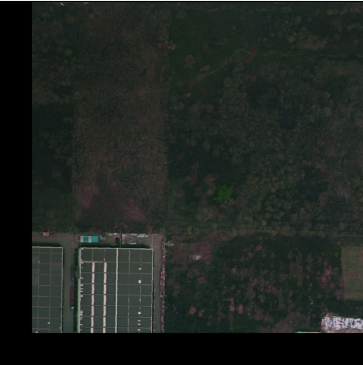
\includegraphics[width=\textwidth]{images/dacs_source_im.png}
                \caption{Source Image}
            \end{subfigure}
            \hspace{2mm}
            \begin{subfigure}[b]{0.4\textwidth}
                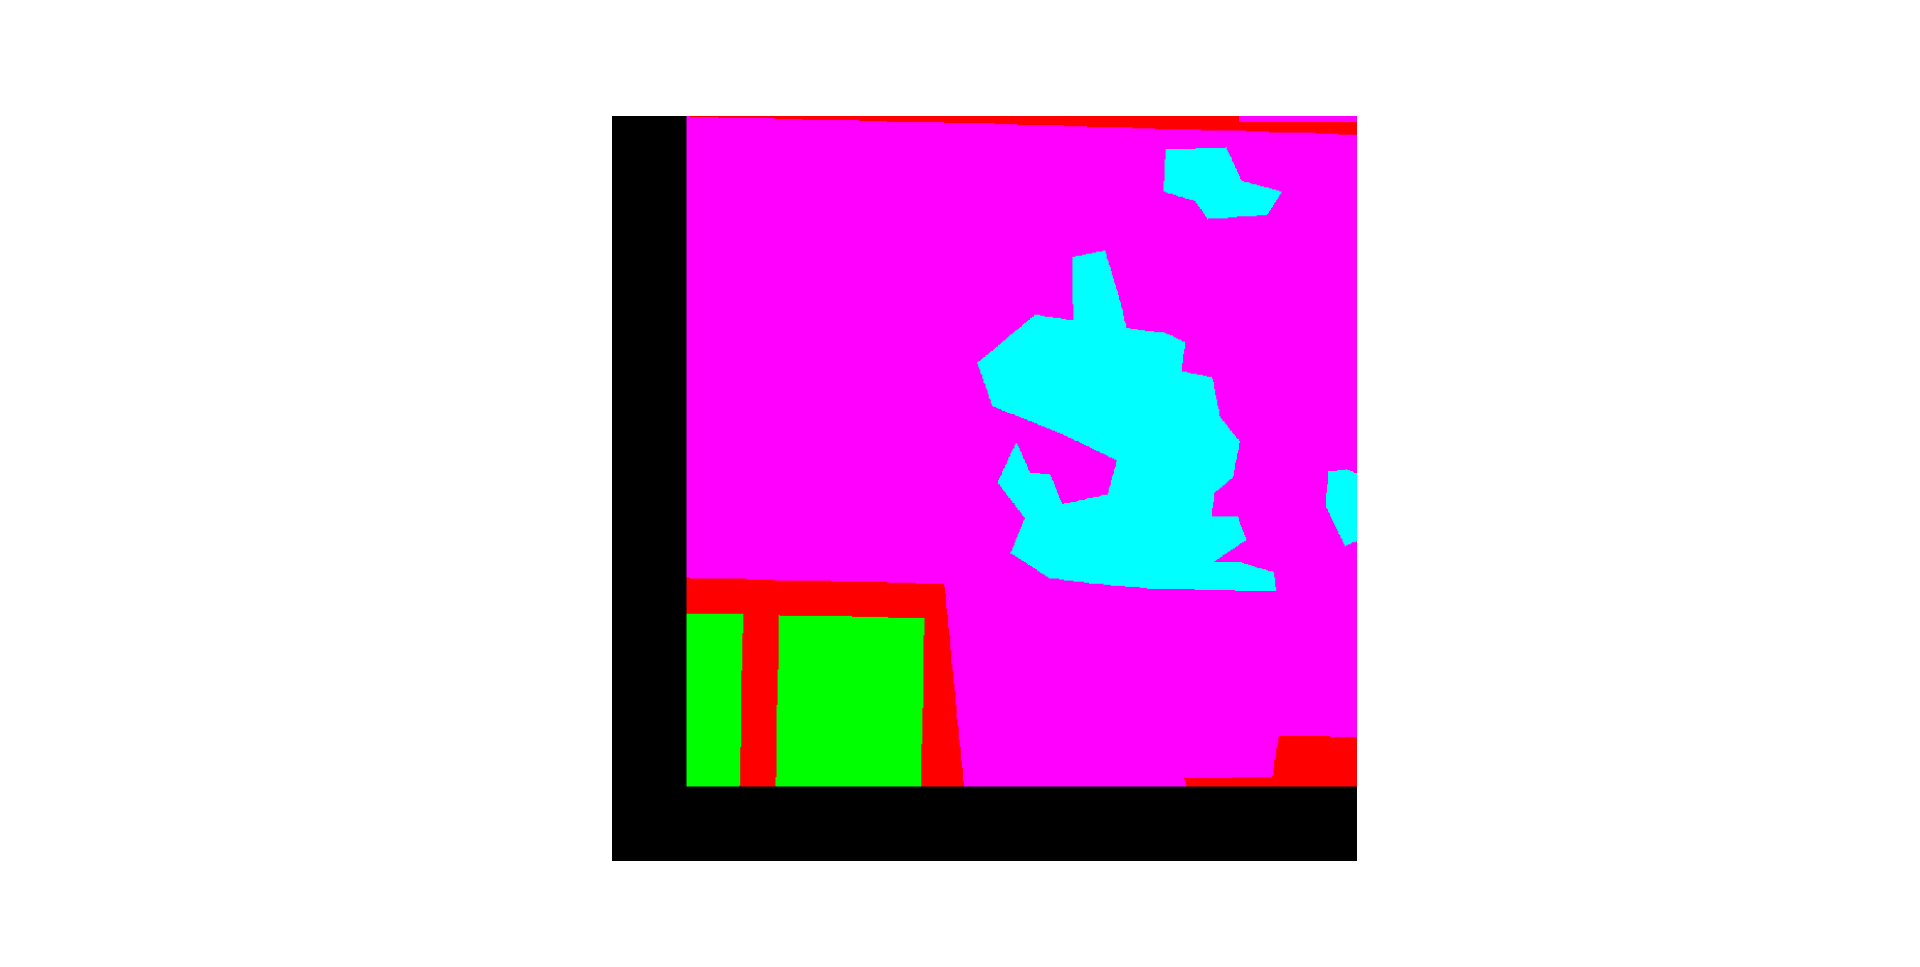
\includegraphics[width=\textwidth]{images/dacs_source_lb.png}
                \caption{Source Label}
            \end{subfigure}
            \vskip\baselineskip
            \begin{subfigure}[b]{0.4\textwidth}
                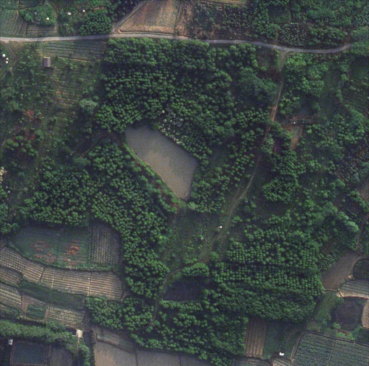
\includegraphics[width=\textwidth]{images/dacs_target_im.png}
                \caption{Target Image}
            \end{subfigure}
            \hspace{2mm}
            \begin{subfigure}[b]{0.4\textwidth}
                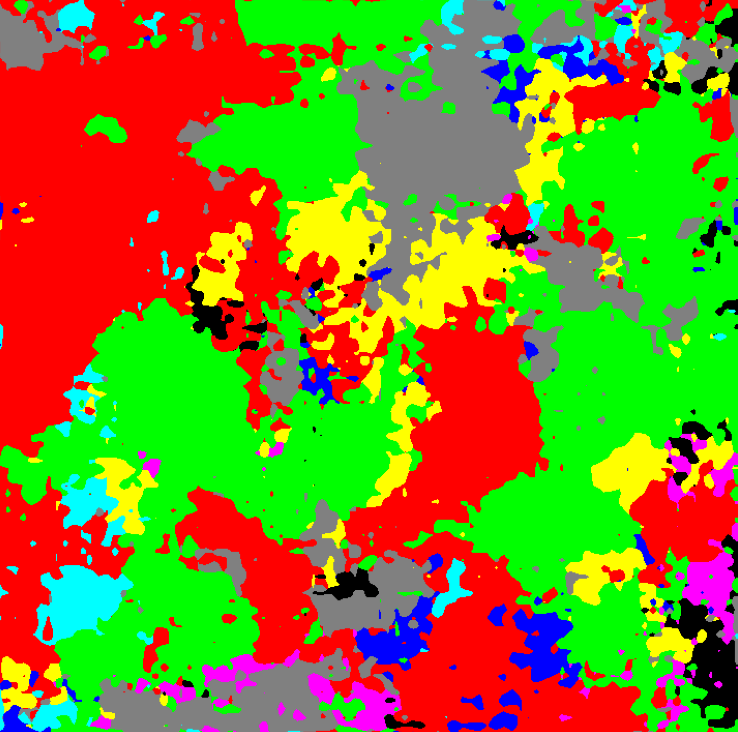
\includegraphics[width=\textwidth]{images/dacs_target_lb.png}
                \caption{Target Pseudo-label}
            \end{subfigure}
            \vskip\baselineskip
            \begin{subfigure}[b]{0.4\textwidth}
                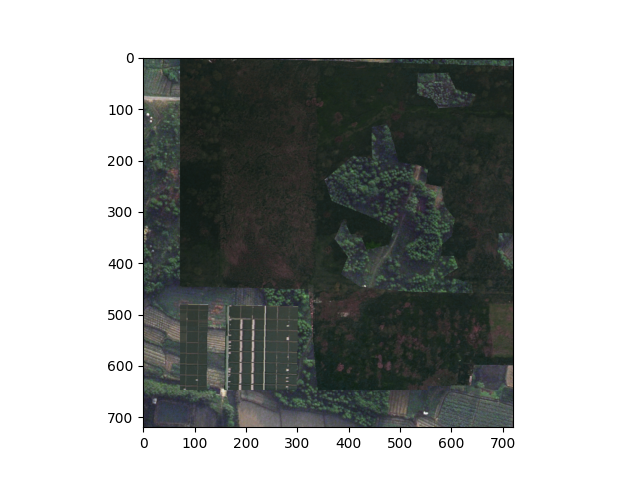
\includegraphics[width=\textwidth]{images/dacs_mixed_im.png}
                \caption{Mixed Image}
            \end{subfigure}
            \hspace{2mm}
            \begin{subfigure}[b]{0.4\textwidth}
                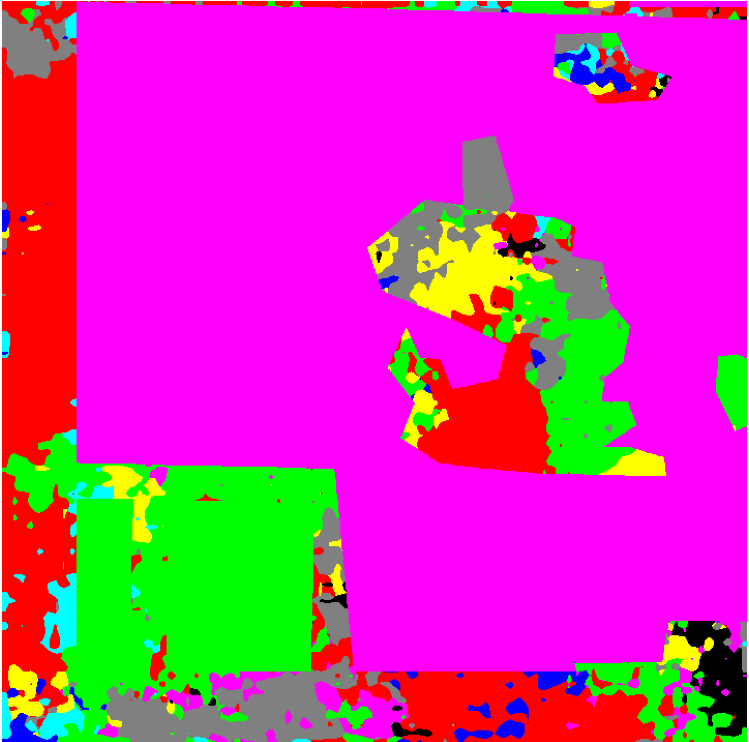
\includegraphics[width=\textwidth]{images/dacs_mixed_lb.png}
                \caption{Mixed Label}
            \end{subfigure}
            \caption{DACS Pictures: Source, Target with Pseudo-labels and Mixed Images}
            \label{fig:DACS}
        \end{minipage}
        \hfill
        \begin{minipage}{0.48\textwidth} 
            \centering
            \captionsetup{font=small}
            \begin{subfigure}[b]{0.4\textwidth}
                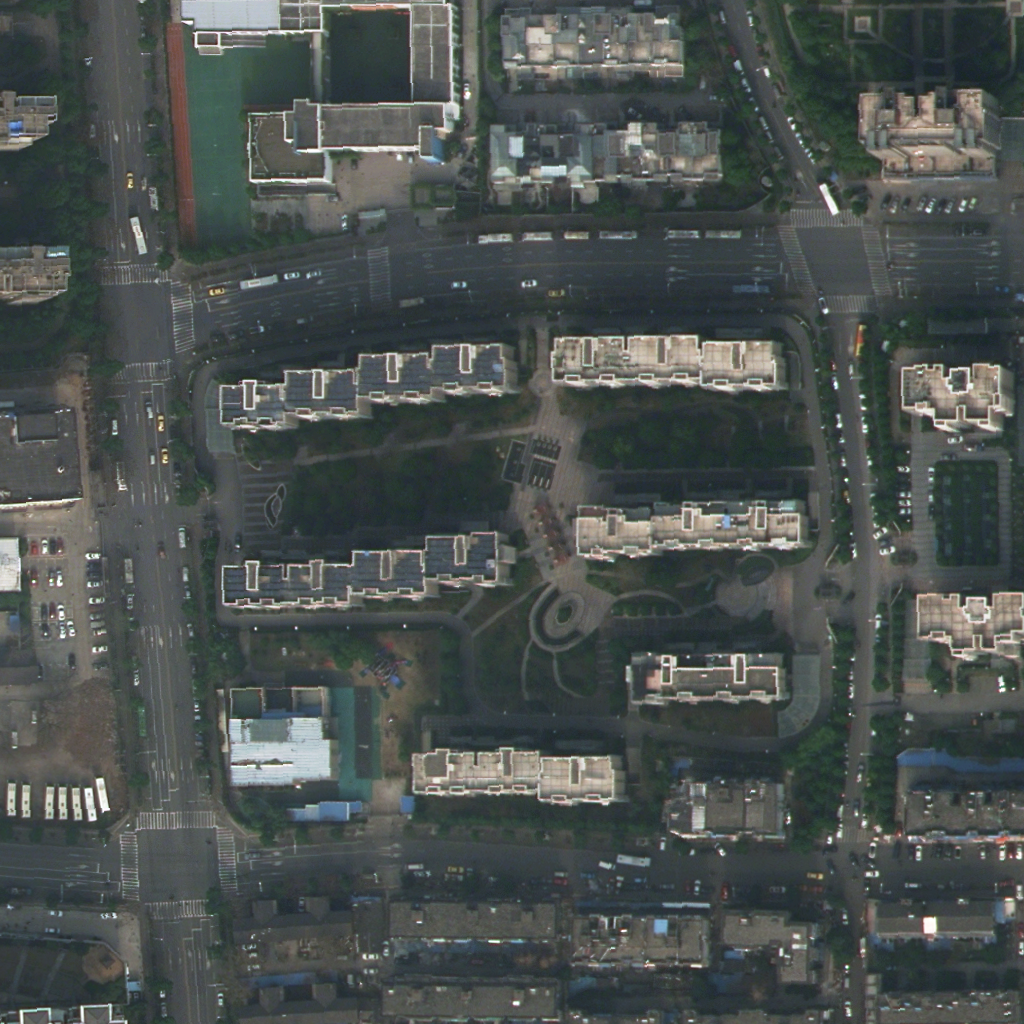
\includegraphics[width=\textwidth]{images/1410.png}
                \caption{Source Image A}
                \label{fig:image1410}
            \end{subfigure}
            \hspace{2mm}
            \begin{subfigure}[b]{0.4\textwidth}
                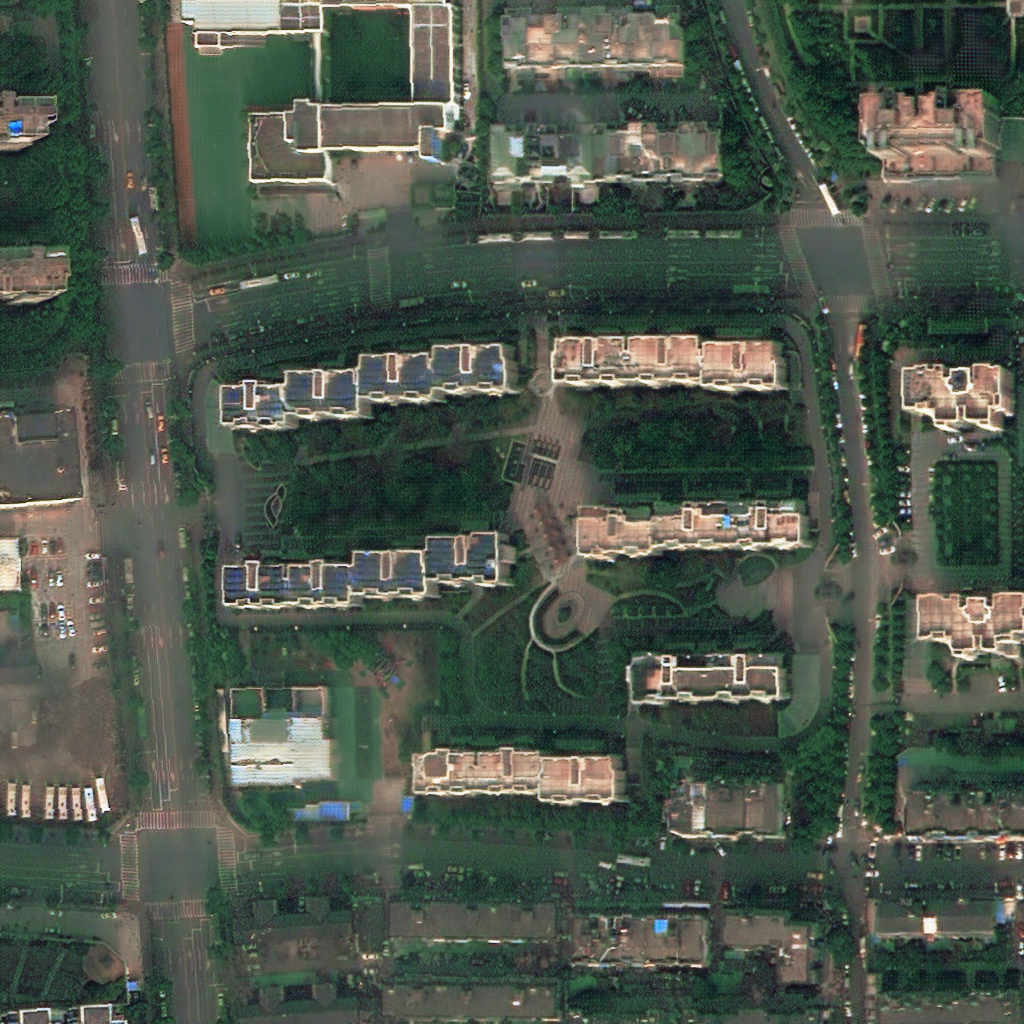
\includegraphics[width=\textwidth]{images/1410_fake.png}
                \caption{CycleGAN Image A}
                \label{fig:image1410_fake}
            \end{subfigure}
            \vskip\baselineskip
            \begin{subfigure}[b]{0.4\textwidth}
                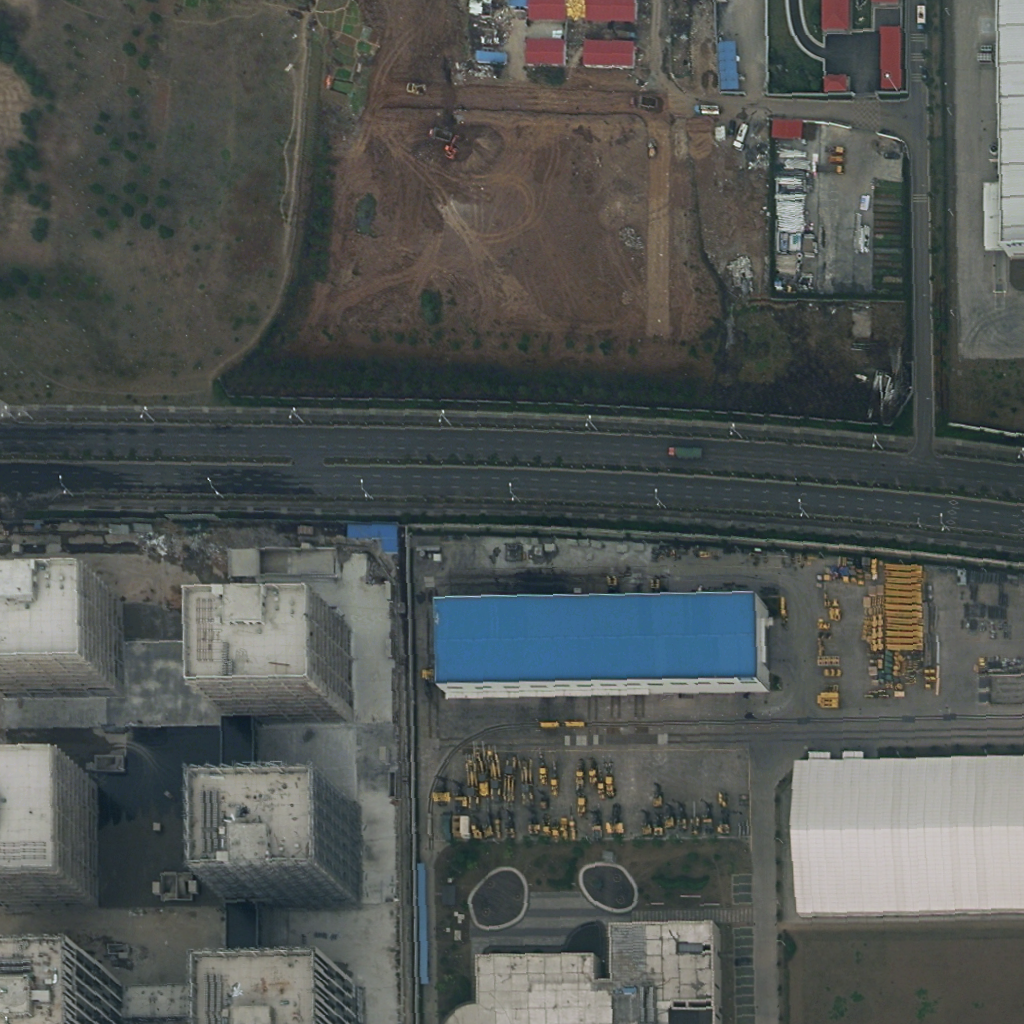
\includegraphics[width=\textwidth]{images/1457.png}
                \caption{Source Image B}
                \label{fig:image1457}
            \end{subfigure}
            \hspace{2mm}
            \begin{subfigure}[b]{0.4\textwidth}
                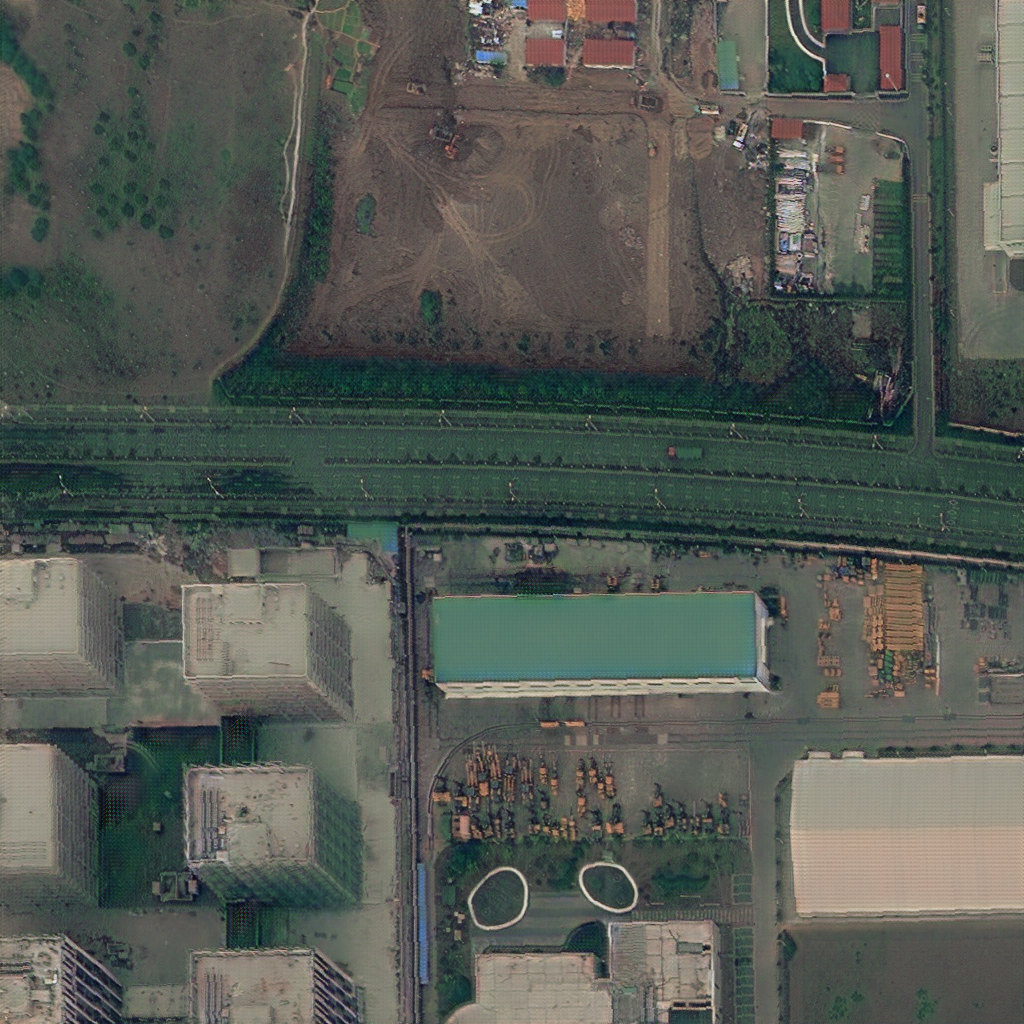
\includegraphics[width=\textwidth]{images/1457_fake.png}
                \caption{CycleGAN Image B}
                \label{fig:image1457_fake}
            \end{subfigure}
            \vskip\baselineskip
            \begin{subfigure}[b]{0.4\textwidth}
                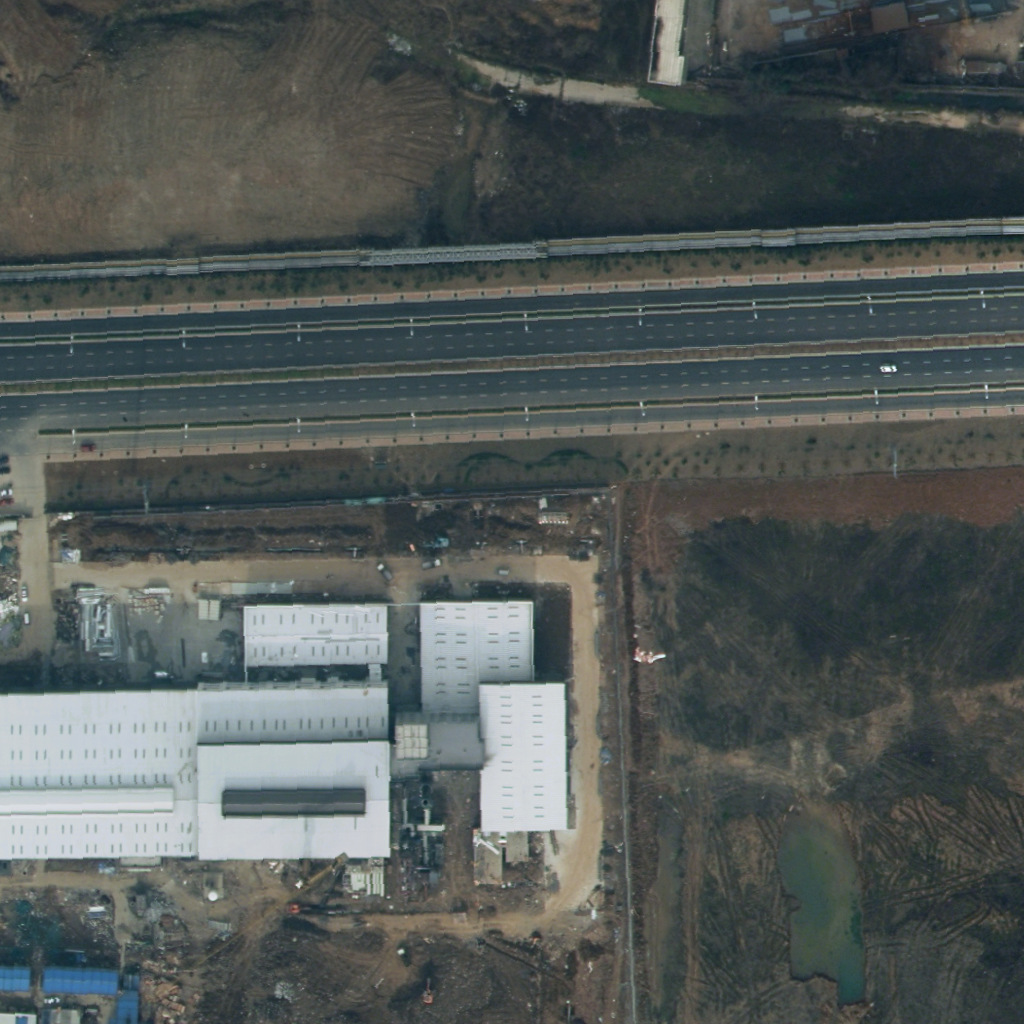
\includegraphics[width=\textwidth]{images/1508.png}
                \caption{Source Image B}
                \label{fig:image1508}
            \end{subfigure}
            \hspace{2mm}
            \begin{subfigure}[b]{0.4\textwidth}
                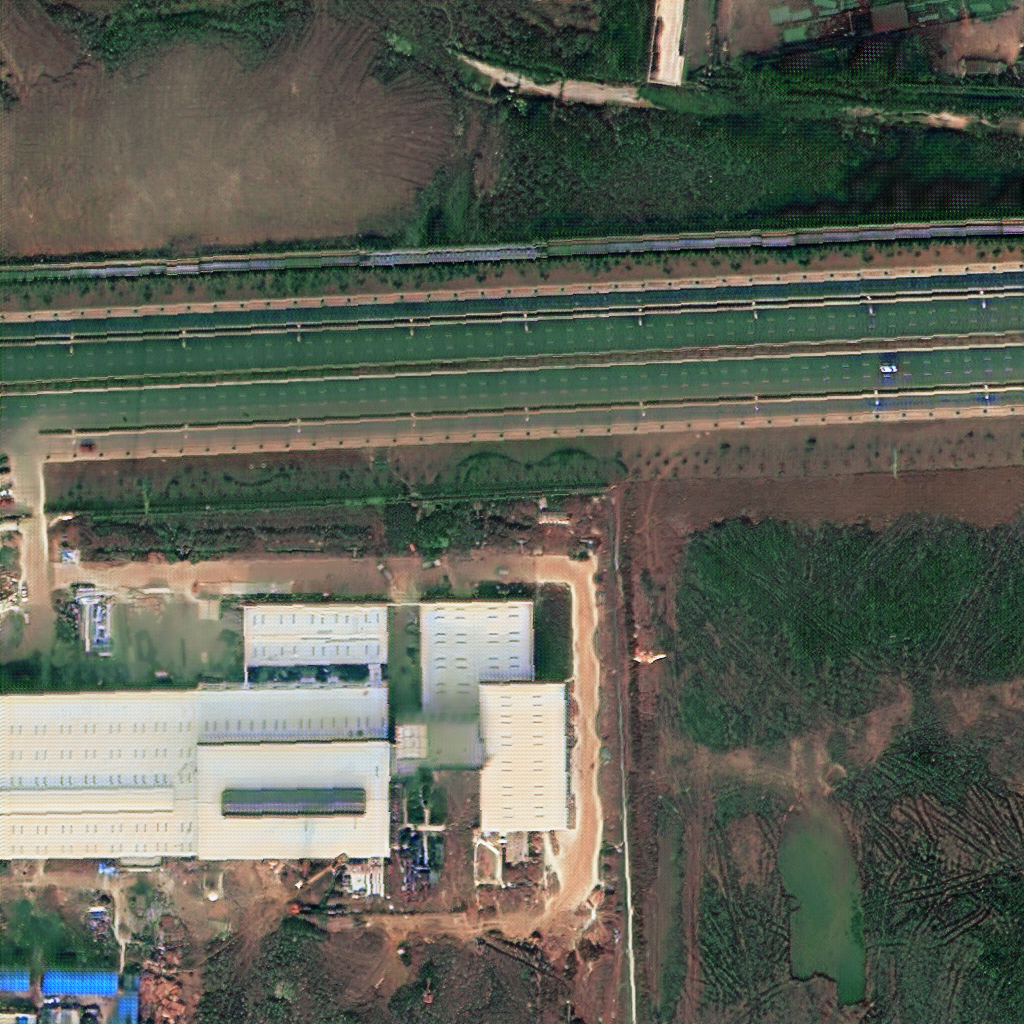
\includegraphics[width=\textwidth]{images/1508_fake.png}
                \caption{CycleGAN Image B}
                \label{fig:image1508_fake}
            \end{subfigure}
            \caption{Comparison between original images and CycleGAN-generated images}
            \label{fig:CycleGAN}  
        \end{minipage}        
    \end{figure*}

    \begin{table*}[t]
    \centering
    \resizebox{1\textwidth}{!}{
    \begin{tabular}{|c|c|c|c|c|c|c|c|c|c|c|c|}
    \hline
    \textbf{Model} & \textbf{Training Set} & \textbf{Target Set} & \textbf{Test Set} & \textbf{mIoU} & \textbf{Building} & \textbf{Road} & \textbf{Water} & \textbf{Barren} & \textbf{Forest} & \textbf{Grassland} & \textbf{Farmland} \\
    \hline
    PIDNet & CycleGAN LoveDa-Urban & LoveDa-Rural & CycleGAN LoveDa-Urban & 0.4035 & 0.3508 & 0.4845 & 0.5442 & 0.6434 & 0.0919 & 0.3659 & 0.3440 \\
    \hline
    PIDNet & CycleGAN LoveDa-Urban & LoveDa-Rural & LoveDa-Rural & 0.2880 & 0.5127 & 0.1962 & 0.3027 & 0.4716 & 0.0625 & 0.0353 & 0.4349 \\
    \hline
    \end{tabular}
    }
    \caption{Performance of PIDNet with CycleGAN-generated Fake Images}
    \end{table*}
}

\subsection{Data Augmentation Experiments}

The previous optimal model was initially tested using LoveDA-Urban as both the source and target domain. However, since this project primarily focuses on Domain Adaptation, we further evaluated the model by training it on the LoveDA-Urban domain and validating it on the LoveDA-Rural domain. The results of this cross-domain evaluation are presented in Table 3.

As outlined in the Methodology section, we implemented four different data augmentation techniques to enhance the PidNet model’s performance in domain adaptation scenarios. Table 3 summarizes the results obtained when applying these techniques to PidNet with the optimal configuration.

The baseline model, trained without any augmentation, achieves a mIoU of 0.2296. Introducing AUG\_CHANCE alone significantly improves performance to 0.2951, demonstrating that increasing dataset diversity helps mitigate domain shift. Among the different augmentation techniques, AUG1, which applies brightness and shadow transformations, enhances road segmentation (0.3789) and farmland (0.4417) but slightly reduces forest performance (0.0377). AUG2, incorporating color shifts and Gaussian blur, achieves an overall mIoU of 0.3108, with notable improvements in barren (0.4075) and grassland (0.1526) classes. AUG3, which consists of geometric transformations, improves building (0.5257) and road (0.3998) segmentation but slightly lowers performance for other classes. 

When augmentations are combined, mixed results are observed. AUG1 combined with AUG2 leads to the best water segmentation (0.3304) and improves grassland (0.1779). The best overall performance is achieved by combining AUG2 and AUG3, resulting in an mIoU of 0.3509, with significant gains in barren (0.4896) and forest (0.1072). On the other hand, applying all augmentation strategies together does not yield significant improvements, suggesting that certain transformations might interfere with each other. 

After analyzing the results, we conclude that AUG2 and AUG3 are the most effective augmentation techniques for enhancing domain adaptation performance in the LoveDA dataset. This configuration will be used for next two experiments, the Adversarial Learning and the DACS.

\subsection{Adversarial Learning Experiments}

The Adversarial Learning technique was implemented to enhance the PIDNet model's performance in domain adaptation scenarios. The model was trained on the LoveDA-Urban domain and tested on the LoveDA-Rural domain to evaluate its ability to generalize across different environments. The results of the experiments are presented in Table 4.
The initialization values used during the training process are critical for balancing the contributions of various components in the adversarial learning setup. Specifically, the learning rates for the first and second discriminators are initializated both equal to $0.0001$. Additionally, the hyperparameters ${\lambda_{seg1}} = 1$, ${\lambda_{seg2}} = 0.01$, ${\lambda_{adv}1} = 0.001$, and ${\lambda_{adv}2} = 0.0002$ are used to control the weights of the segmentation loss and adversarial losses. 
The experimental results demonstrate that the baseline PIDNet model achieves an mIoU of 0.3509 when tested on the LoveDA-Rural domain, while the adversarial multi-state variant (PIDNet-ADV) shows a decrease in performance with an mIoU of 0.2770. The class-wise analysis reveals that PIDNet maintains superior performance across most categories, with notable advantages in Barren (+10.88\%), Water (+7.28\%), and particularly Grassland (+22.80\%). However, PIDNet-ADV exhibits marginally better performance in Forest class (+2.34\%). This performance degradation in the adversarial variant suggests that while adversarial training might enhance robustness, it could potentially compromise the model's ability to generalize effectively across domain shifts, particularly in the challenging urban-to-rural transfer scenario characteristic of the LoveDA dataset.

\subsection{DACS Experiments}

The same experiments done on Adversarial Learning was done also on Image-to-Image approach with DACS. The results obtained with PIDNet using DACS (presented in Table 4) demonstrate a notable improvement compared to some of the previous configurations without DACS. The mIoU reaches 0.2918, surpassing the baseline (0.2296) and some configurations that relied solely on data augmentation. This suggests that DACS effectively enhances domain adaptation by leveraging pseudo-labels to refine feature alignment between the source and target domains. Compared to the best augmentation-based configuration (AUG2 + AUG3, mIoU = 0.3509), DACS still underperforms slightly, particularly in barren (0.4343 vs. 0.4896) and forest (0.1016 vs. 0.1072) regions, but achieves competitive performance in water (0.2913 vs. 0.3407) and grassland (0.2310 vs. 0.2865).
Notably, DACS significantly improves farmland segmentation (0.3959) compared to augmentation-based methods, which struggled with this class. It also yields a strong improvement in building (0.5454) and road (0.3345) segmentation, reinforcing its capability to enhance structured urban features. However, the overall performance remains below the optimal augmentation-only strategy (0.3509), indicating that pseudo-labels may still introduce some noise, especially in complex, texture-rich rural landscapes. 

The Figure 1 shows the source image, the source label associated, the target image and the pseudo-label generated and the mixed image and the corresponsing mixed label of a single iteraction. 

\subsection{CycleGAN Experiments}

The CycleGAN model was employed to generate synthetic datasets aimed at bridging the domain gap between the urban and rural environments in the LoveDA dataset. The Generator networks are based on the ResNet architecture to mitigate the vanishing gradient problem, while the Discriminator networks utilize a basic CNN architecture. The least-squares loss function is used as the adversarial loss to stabilize training, and an image pool mechanism is adopted to store previously generated fake images. This prevents the discriminators from overfitting to recent examples. The optimizer used is Adam with a batch size of 1 and a learning rate of 0.0002. The model was trained for 27 epochs. 

After training, only the generator transforming Urban $\Rightarrow$ Rural is utilized to create a synthetic "fake rural" dataset from the Urban training images. Examples of these synthetic images are shown in Figure 2. PIDNet was subsequently trained using two configurations: (1) training and validation on CycleGAN-transformed Urban images, and (2) training on CycleGAN-transformed Urban images and validation on the original Rural images. Table~5 summarizes the results of these experiments.

The results demonstrate that CycleGAN-generated images fail to provide meaningful domain adaptation for the LoveDA dataset. In the first configuration, PIDNet achieves a mean Intersection over Union (mIoU) of 0.4035, which is lower than the baseline mIoU. Similarly, in the second configuration, the mIoU drops further to 0.2880 when validated on the Rural domain. Class-wise analysis reveals significant inconsistencies, with especially poor performance in the Forest, Grassland, and Farmland categories in the second configuration. For example, Grassland achieves an mIoU of only 0.0353, indicating the inability of CycleGAN to capture the unique characteristics of the rural domain. 

These results suggest that CycleGAN's transformation from Urban to Rural images introduces substantial bias, resulting in synthetic images that do not accurately reflect the true rural domain distribution. Consequently, training PIDNet on these biased synthetic datasets fails to improve segmentation performance. This highlights the limitations of using CycleGAN in scenarios where significant class distribution differences exist between domains, as it struggles to capture the full variability of the target domain.




\subsection{PEM Experiments}
The experiments done with PEM model can be seen in Table 6. The PEM model achieves an mIoU of 0.4685 when trained on CycleGAN-transformed LoveDA-Urban data and tested on LoveDA-Rural, outperforming both PIDNet variants in the same cross-domain scenario. Specifically, PIDNet with CycleGAN-transformed training data achieves an mIoU of 0.2880, while the augmented PIDNet reaches an mIoU of 0.3509. This suggests that PEM's architecture might be more effective at leveraging CycleGAN-transformed data for domain adaptation compared to PIDNet. For reference, PEM's performance on single-domain scenarios shows an mIoU of 0.6444 for urban and 0.4459 for rural environments, highlighting the inherent challenges in rural scene segmentation regardless of the adaptation strategy employed.

\begin{table}[H]
\centering
\resizebox{1\columnwidth}{!}{
\begin{tabular}{|c|c|c|c|c|}
\hline
\textbf{Model} & \textbf{Training Set} & \textbf{Test Set} & \textbf{mIoU} & \textbf{mACC}  \\
\hline
PEM-URBAN & LoveDa-Urban & LoveDa-Urban & 0.6444  & 75.1795  \\
\hline
PEM-RURAL & LoveDa-Urban  & LoveDa-Rural & 0.4458 & 54.6906  \\
\hline
PEM-CycleGAN & CycleGAN LoveDa-Urban & LoveDa-Rural & 0.4685 & 62.2863 \\
\hline
\end{tabular}
}
\caption{Performance of PEM Model with Different Training and Test Sets}
\end{table}


\section{Conclusion}

In this project, we explored various methodologies to enhance the performance of semantic segmentation models in domain adaptation scenarios. We evaluated the DeepLabV2 and PIDNet models on the LoveDA dataset, focusing on urban-to-urban evaluation to compare the performance of a real-time segmentation model and a non-real-time segmentation model. Our experiments revealed that PIDNet, configured with the Adam optimizer, OCE loss, a learning rate scheduler, and a resolution of 720×720, achieved the best performance with an mIoU of 0.4368, outperforming all other PIDNet and DeepLabV2 configurations. However, for the domain adaptation task, this PIDNet configuration encountered difficulties, achieving an mIoU of only 0.2296. Data augmentation techniques, particularly AUG2 and AUG3, significantly improved segmentation quality in the cross-domain adaptation scenario, with an mIoU of 0.3509, demonstrating the importance of dataset diversity in domain adaptation. Conversely, adversarial learning and DACS did not yield the expected improvements, suggesting that these techniques may not be well-suited for the LoveDA dataset. PEM, a transformer-based architecture, outperformed PIDNet in domain adaptation, achieving an mIoU of 0.4685, highlighting the potential of transformer-based models in addressing domain shifts. Finally, CycleGAN-generated fake images were used to train PIDNet, resulting in an mIoU of 0.2880. While CycleGAN improved the performance compared to the baseline model (without augmentations), it failed to outperform configurations with data augmentation applied.


\bibliographystyle{unsrt}
\bibliography{references}

\end{document}